% !TeX spellcheck = pt_BR
\documentclass[aspectratio=169, xcolor=dvipsnames]{beamer}
%Definições de tema
\setbeamertemplate{blocks}[rounded][shadow=false]
\usetheme{Madrid}
\setbeamertemplate{items}[square]
\setbeamertemplate{caption}[numbered]
\usecolortheme{beaver}
\setbeamercolor{frametitle}{bg=white!10!white}

\usefonttheme{professionalfonts}
\setbeamertemplate{itemize item}{\color[rgb]{0.8,0,0}$\blacksquare$}
\setbeamertemplate{itemize subitem}{\color[rgb]{0.8,0,0}$\blacksquare$}
\setbeamertemplate{itemize subsubitem}{\color[rgb]{0.8,0,0}$\blacksquare$}

%Definições de seção
\setcounter{secnumdepth}{3}
\setcounter{tocdepth}{2}


\usepackage{xkeyval}
\usepackage{todonotes}
\presetkeys{todonotes}{inline}{}


\usepackage{helvet}
\renewcommand{\familydefault}{\sfdefault}
\usepackage{float}
\usepackage[brazil]{babel}
\usepackage[utf8]{inputenc}
\usepackage{graphicx, tikz}
\usepackage{url}
\usepackage{subfigure}
\usepackage{mathtools} % setas com texto
\usepackage{multicol}
\usepackage{listings}
\usepackage{lipsum}
\usepackage{scalefnt}
\usepackage{ragged2e}
\usepackage{etoolbox, verbatim}

% Listing
\lstset{
	numbers=left,
	stepnumber=1,
	numbersep=6pt,
	numberstyle=\small\color{black},
	basicstyle= \scriptsize,
%	keywordstyle=\color{black},
%	commentstyle=\color{black},
%	stringstyle=\color{black},
	tabsize=2
}
%Definições Listing - Linguagem Scala
\lstdefinelanguage{scala}{
morekeywords={abstract,case,catch,class,def,%
	do,else,extends,false,final,finally,%
	for,if,implicit,import,match,mixin,%
	new,null,object,override,package,%
	private,protected,requires,return,sealed,%
	super,this,throw,trait,true,try,%
	type,val,var,while,with,yield},
otherkeywords={=>,<-,<\%,<:,>:,\#,@},
sensitive=true,
morecomment=[l]{//},
morecomment=[n]{/*}{*/},
morestring=[b]",
morestring=[b]',
morestring=[b]"""
}

\let\olditem=\item%
\renewcommand{\item}{\olditem \justifying}

\title[Processamento Digital de Imagem - \textit{Face Detection}]{\textbf{Processamento Digital de Imagem}\\\textit{Face Detection - Referencial Teórico parte 2}}
\author[rodolfolabiapari@decom.ufop.br]{Rodolfo Labiapari Mansur Guimarães}
\institute[IFMG]{\begin{figure}
			\centering
			
\includegraphics[width=0.1\textwidth]{img/ufop.jpg}
		\end{figure}}
\institute[UFOP]{
	\textit{rodolfolabiapari@decom.ufop.br} \\
	Lattes: \url{http://goo.gl/MZv4Dc} \\
	Departamento de Computação -- Universidade Federal de Ouro Preto \\
	Ouro Preto - MG -- Brasil }

\date[\today]{Última Atualização: \today.}

\begin{document}


\frame{\titlepage}

\AtBeginSection[]
{
	\begin{frame}
	\frametitle{Sumário}
	\tableofcontents[]
	\end{frame}
}

\AtBeginSubsection[]
{
	\begin{frame}
	\frametitle{Sumário}
	\tableofcontents[
    currentsection,
    currentsubsection,
    hideothersubsections,
    %sectionstyle=show/hiden,
    subsectionstyle=show/shaded, ]
	\end{frame}
}

%\usebackgroundtemplate{
\includegraphics[trim=0cm 0cm 10cm 0cm, width=0.03\textwidth]{img/ufop.jpg}}

\section{Introdução}
	\subsection{Apresentação}
	\begin{frame}{Apresentação}
		\begin{itemize}
			\setlength\itemsep{2em}
			\item Pesquisas recentemente buscam procedimentos que focam em \textbf{detecção de face} em ambientes onde existe uma \textbf{maior complexidade}, sem perder sua \textbf{eficiência}.

			\item As maiores dificuldades atuais são
			\begin{itemize}
				\setlength\itemsep{1.5em}
				\item Larga variações de visualização de faces humanas em fundos não-padronizados; e também
				\item A procura espacial onde cada face pode estar posicionada em diferentes posições e tamanhos  \cite{Haoxiang2015}.
			\end{itemize}
		\end{itemize}
	\end{frame}

	\subsection{Justificativa}
	\begin{frame}{Justificativa}
		\begin{itemize}
			\setlength\itemsep{2em}
			\item Sistemas computacionais \textbf{anteriores à redes neurais} possuíam resultados bastante \textbf{ineficientes} para imagens que tinham como propriedade fundos com complexidade elevada.

			\item Sucesso de algoritmos que utilizam técnicas como a \textit{convolutional neural network} (CNN) \cite{Haoxiang2015}.
		\end{itemize}
	\end{frame}

	\subsection{Referencial Teórico}
		\subsubsection{Reconhecimento de Objetos utilizando Neural Networks}
		\begin{frame}[allowframebreaks]{Reconhecimento Utilizando Neural Networks -}
			\begin{itemize}
				\item Redes neurais comuns proposta inicialmente por McCulloch e Pitts \cite{McCulloch1943} \cite{Bengio-2009}.

				\begin{figure}[h]
					\centering
					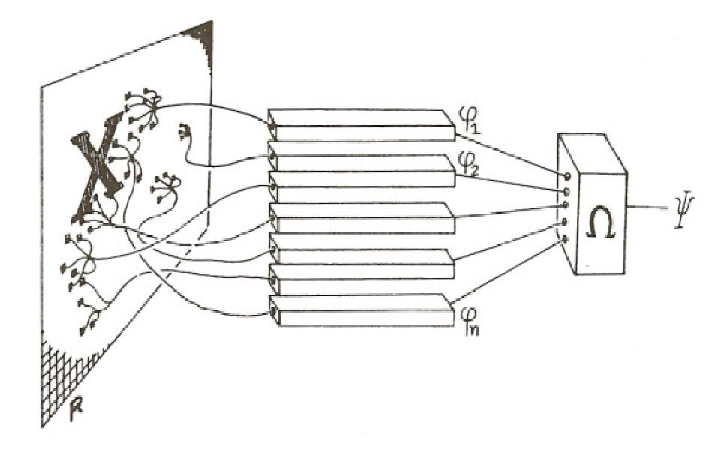
\includegraphics[width=0.5\linewidth]{img/single_layer_cnn.png}
					\caption{Rede neural de arquitetura tipo \textit{feed-forward neural network}.}
					\label{fig:single_layer_cnn.png}
				\end{figure}

				\item Inicialmente utilizava algoritmos de \textit{backpropagation}

				\begin{figure}[h]
					\centering
					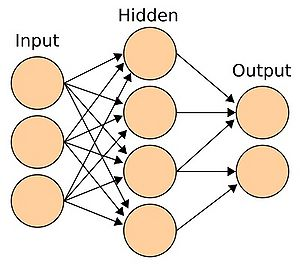
\includegraphics[width=0.4\linewidth]{img/ffnn.jpg}
					\caption{Rede neural FFNN simples.}
					\label{fig:ffnn.jpg}
				\end{figure}

				\setlength\itemsep{2em}
				\item A ativação de determinado neurônio dar-se pelo \textbf{processo de somatório de pesos}
				\begin{itemize}
					\item Os números de neurônios e seus cálculos \textbf{podem crescer exponencialmente} com facilidade em relação à sua entrada.

				\end{itemize}

				\item A \textit{feed-forward neural network} (FFNN) \textbf{não é prática} para vários tipos de problemas reais da computação \cite{Glorot2010}.

			\end{itemize}
		\end{frame}

		\subsubsection{Proposta da Arquitetura Convolutional Neural Network}
		\begin{frame}[allowframebreaks]{Proposta da Arquitetura Convolutional Neural Network -}
			\begin{itemize}
				\setlength\itemsep{2em}
				\item Explora a correlação espacial reforçando:
				\begin{itemize}
					\setlength\itemsep{1em}
					\item Um padrão de conectividade local entre neurônios nas camadas adjacentes.
				\end{itemize}

				\item As entradas da camada $ m $ são de um conjunto da camada anterior $ m-1 $ relacionados de uma forma contígua \cite{LeCun1998}.

					\begin{figure}[H]
						\centering
						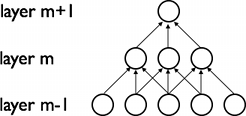
\includegraphics[width=0.45\linewidth]{img/layers_cnn.png}
						\caption{Exemplo das camadas de uma rede \textit{convolutional neural network}.}
						\label{fig:layers_cnn}
					\end{figure}

				\item O algoritmo baseia-se em vários pequenos processos. São eles a
				\begin{itemize}
					\item \textit{Convolution};
					\item \textit{Subsampling}; e a
					\item Mescla dos dois processos.
				\end{itemize}

				\item O processo de \textbf{Convolution} trata-se da prática de aplicar repetidas vezes a saída de determinada função como entrada de outra.

				\item \textbf{Subsampling} utiliza o algoritmo de \textit{max\_pooling}
				\begin{itemize}
					\item  Reduz o tamanho de amostras a ser processada \cite{Giusti2013}.
				\end{itemize}
			\end{itemize}
		\end{frame}


\section{Estudo} \label{sec:desenvolvimento}

	\subsection{Procedimentos de Operação de uma Convolutional Neural Network}
	\begin{comment}

			\begin{frame}[allowframebreaks]{Operação de uma Convolutional Neural Network -}
				\begin{figure}[H]
					\centering
					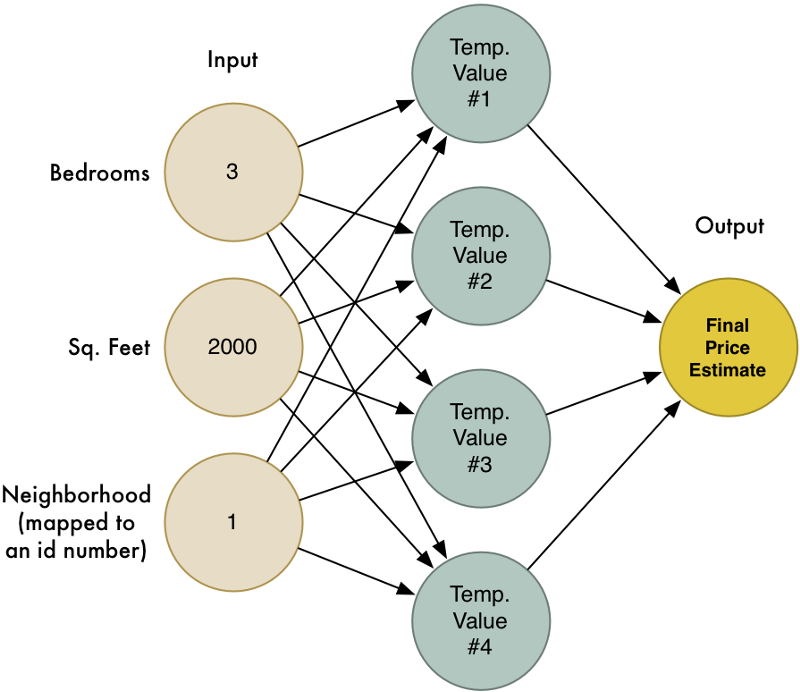
\includegraphics[width=0.4\linewidth]{img/simple_neural.png}
					\caption{Rede neural simples para um problema computacional complexo. Exemplo de um estimador de preço de casa.}
					\label{fig:simple_neural}
				\end{figure}

				\begin{itemize}
					\item Treinamento
				\end{itemize}

				\begin{figure}[t]
					\centering
					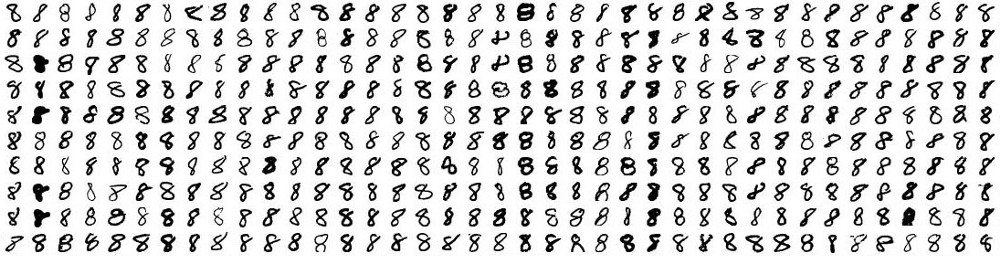
\includegraphics[width=1\linewidth]{img/entrada_padrao_8.jpeg}
					\caption{Exemplo de treinamento do algoritmo utilizando vários formatos de 8 escritos à mão livre.}
					\label{fig:entrada_padrao_8}
				\end{figure}


				\begin{itemize}
					\item Tem-se inúmeras possíveis entradas/escritas do valor 8.
					\begin{itemize}
						\setlength\itemsep{1em}
						\item Usando um padrão de entrada sendo uma imagem 18x18, temos um total de 324 pixels;
						\item Dessa forma, nosso algoritmo passa de 3 para 324 entradas.
					\end{itemize}
				\end{itemize}

				\begin{figure}[H]
					\centering
					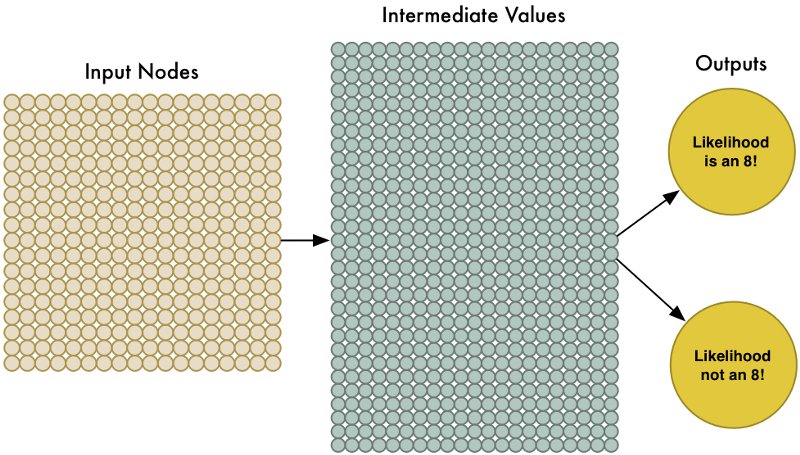
\includegraphics[width=0.78\linewidth]{img/visao_gera_8.png}
					\caption{Visão geral do sistema descrito.}
					\label{fig:visao_geral_8}
				\end{figure}
			\end{frame}
	\end{comment}

	\subsubsection{Enquadramento da Imagem}
	\begin{frame}[allowframebreaks]{Enquadramento da Imagem -}
		\begin{itemize}
			\setlength\itemsep{1.2em}
			\item \textbf{Busca utilizando Janela Deslizante:} Uma máscara que percorre toda a imagem.

			\item \textbf{Utilização de dados mais variantes:} Como a imagem pode estar com com uma posição diferente, permite-se então a criação de outra técnica que \textit{procura mais dados com posições variantes}.

			\item \textbf{Convolução:}
				\begin{enumerate}
					\setlength\itemsep{0.8em}
					\item Quebra-se a imagem em vários quadros.
					\item Utiliza-se cada quadro em uma \textbf{pequena rede neural}. Os resultados serão salvos numa matriz que segue a indexação da imagem original.
					\item A matriz de resultados final será avaliada com algoritmo de \texttt{max\_pooling} e este processo chama-se \textit{Redução de Amostragem}.
				\end{enumerate}

			\item Com esse processo, elimina-se os itens irrelevantes para o processamento.

			\begin{figure}[H]
				\centering
				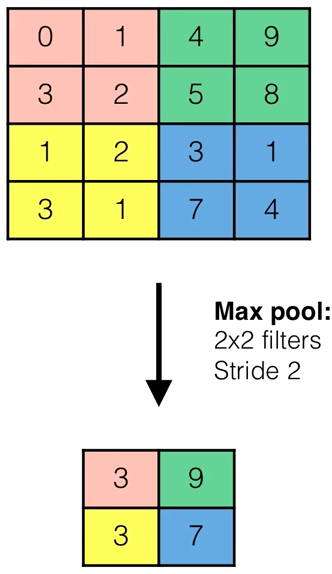
\includegraphics[width=0.2\linewidth]{img/max_pooling.png}
				\caption{O processo de seleção de melhores resultados. Procedimento executado pela função \texttt{max\_pooling}.}
				\label{fig:max_pooling.png}
			\end{figure}

			\item Os itens resultantes serão entrada para outra rede neural

			\item Fará de fato a decisão final.

				\vspace{100px}

			\begin{figure}[h]
				\centering
				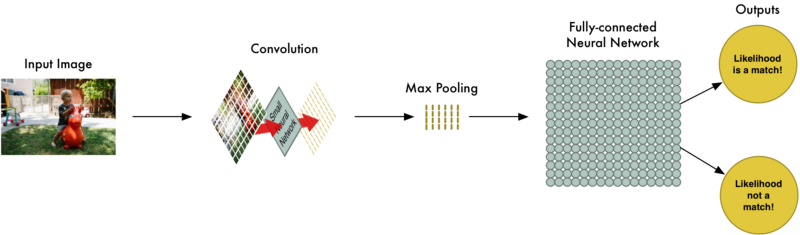
\includegraphics[width=1.0\linewidth]{img/convolucao_teoria.png}
				\caption{O processo simples de uma arquitetura de reconhecimento de padrão \textit{convolutional neural network} final após todos os processos.}
				\label{fig:convolucao_teoria}
			\end{figure}
		\end{itemize}
	\end{frame}


	\subsection{Data Set}
	\begin{frame}{Data Set}

		\begin{multicols*}{2}

			\begin{itemize}
				\item \textit{Benchmark} disponibilizado gratuitamente pela Universidade de Massachusets Amherst \cite{fddbTech}.
			\end{itemize}

			\begin{figure}[H]
				\centering
				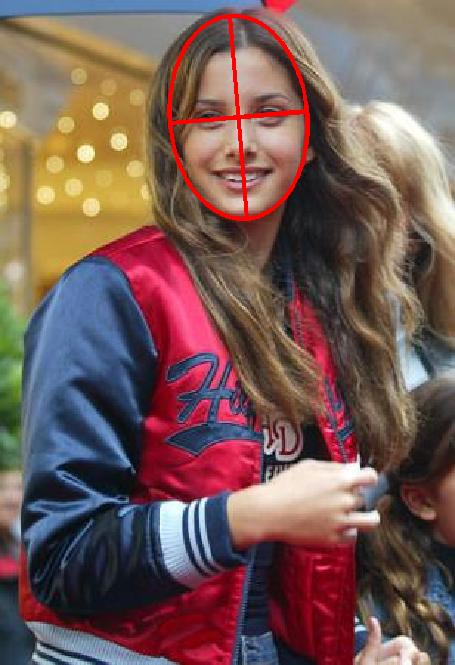
\includegraphics[width=0.52\linewidth]{img/data_set.jpg}
				\caption{Exemplo de identificação de rosto especificado pelo \textit{data-set} disponibilizado pela Universidade de Massachusets Amherst.}
				\label{fig:mulher}
			\end{figure}
		\end{multicols*}
	\end{frame}

\frame{\titlepage}

\bibliographystyle{sbc}
\bibliography{example}

\frame{\titlepage}


\end{document}
